\documentclass[a4paper,12pt]{article}
\usepackage[a4paper,left=3cm,right=2cm,top=2.5cm,bottom=2.5cm]{geometry}
\usepackage[utf8]{inputenc}
\usepackage{graphicx}
\usepackage[table]{xcolor}
\usepackage{array}
\usepackage{float}
\usepackage{enumitem}
\usepackage{hyperref}
\hypersetup{hidelinks}
\usepackage{amsmath}
\usepackage[ruled,vlined,linesnumbered,algoruled]{algorithm2e}
\usepackage{tabularx}

% Define subsubsubsection
\makeatletter
\newcommand\subsubsubsection{\@startsection{subsubsubsection}{4}{\z@}%
	{-3.25ex\@plus -1ex \@minus -.2ex}%
	{1.5ex \@plus .2ex}%
	{\normalfont\normalsize\bfseries}}
\newcommand*{\subsubsubsectionmark}[1]{}
\makeatother

% Dades de la pràctica
\newcommand{\titolPractica}{Supermaket Manager: \textbf{Manual d'Uusari}}
\newcommand{\identificadorEquip}{Subrgrup 11.3}
\newcommand{\PROPquatrimestre}{PROP - Quadrimestre de tardor 2024}
\newcommand{\versioLliurament}{Versió del lliurament 3.0}

% Dades de renovar comandes
\renewcommand*\contentsname{Continguts}
\renewcommand{\figurename}{Figura}
\renewcommand{\tablename}{Taula}

\begin{document}
	
	% Tapa del document
	\begin{titlepage}
		\begin{center}
			{\Large \textbf{\titolPractica}} \\[10cm]
			\textbf{\large \identificadorEquip} \\[1cm]
			Guillem Cabré Farré, \small{@guillem.cabre} \\
			Marc Peñalver Guilera, \small{@marc.penalver} \\
			Àlex Rodríguez Rodríguez, \small{@alex.rodriguez.r} \\
			Marc Teixidó Sala, \small{@marc.teixido} \\[2cm]
			\textbf{\versioLliurament} \\
			\textbf{\PROPquatrimestre} \\
			\textbf{Data: \today}
		\end{center}
	\end{titlepage}
	
	% Índex de continguts
	\tableofcontents
	\clearpage
	
	\section{Introducció}
	\subsection{Objectiu del manual}
	Aquest manual té com a finalitat guiar l'usuari en l'ús del programa \textbf{Supermarket Manager}, desenvolupat pel subgrup 11.3 en el marc del projecte PROP del quadrimestre de tardor del 2024. Proporciona instruccions detallades per configurar, operar i treure el màxim profit de l'aplicació.
	
	\subsection{Descripció general del programa}
	El \textbf{Supermarket Manager} és una aplicació dissenyada per optimitzar la gestió dels productes en un supermercat. El programa permet:
	\begin{itemize}
		\item Administrar el catàleg de productes, incloent-hi la seva importació i exportació des de fitxers JSON.
		\item Organitzar els productes a les prestatgeries de forma manual o mitjançant algorismes especialitzats.
		\item Visualitzar i gestionar la distribució dels productes, tenint en compte les seves restriccions de temperatura.
	\end{itemize}
	Aquest manual està dirigit a administradors i empleats del supermercat, amb o sense experiència prèvia en gestió informàtica.
	
	\newpage
	\section{Interfície d'usuari}
	
	El programa informàtic té un total de 5 pantalles que permeten a l'usuari navegar entre diferents funcionalitats i modes d'operació. A continuació detallarem cada una d'elles. \\
	
	Cal tenir en compte que el supermercat utilitzarà símbols per referir-se a les diferents temperatures que poden adoptar tant les prestatgeries com els productes. Aquests símbols són:
	
	\begin{center}
		
\includegraphics[width=0.1\textwidth]{assets/AMBIENT.png} % Exemple d'altre símbol
		\hspace{1cm}
		
\includegraphics[width=0.1\textwidth]{assets/REFRIGERATED.png} % Ajusta el camí i la mida
		\hspace{1cm} % Espai entre imatges
		
\includegraphics[width=0.1\textwidth]{assets/FROZEN.png} % Exemple d'altre símbol
	\end{center}
	
	Aquestes imatges simbolitzen en ordre: temperatura ambient, temperatura de nevera i temperatura de congelador. Aquests apareixeran a sobre de cada prestatgeria de la interfície.
	
	\newpage
	\subsection{Log In}
	\label{sec:logIn}
	
	Aquesta finestra permet iniciar sessió tant a l'empleat com a l'administrador. Per defecte, la contrasenya d'ambdós perfils és la següent:
	
	\begin{itemize}
		\item \textbf{Administrador}: nom d'usuari \texttt{admin}, contrasenya \texttt{admin}.
		\item \textbf{Empleat}: nom d'usuari \texttt{employee}, contrasenya \texttt{employee}.
	\end{itemize}
	
	A la figura següent es pot observar la interfície de l'inici de sessió. Tot seguit, es detallen les funcionalitats disponibles.
	
	\begin{figure}[H] 
		\centering
		\includegraphics[width=0.75\linewidth]{assets/login.png}
		\caption{Interfície de Log In}
	\end{figure}
	
	\noindent Les funcionalitats de la vista són:
	
	\begin{enumerate}[itemsep=0pt, topsep=0pt]
		\item Camp d'entrada per introduir el nom d'usuari.
		\item Camp d'entrada per introduir la contrasenya.
		\item Botó de confirmació per validar les dades introduïdes. Navegarem a \textit{Main Screen} (\ref{sec:mainScreen}).
		\item Botó de tancament per sortir de l'aplicació o finalitzar la sessió activa.
	\end{enumerate}
	
	\newpage
	\subsection{Main Screen}
	\label{sec:mainScreen}
	
	Aquesta és la vista arrel, des de la que arribarem a totes les demès. La seva principal funcionalitat és mostrar la distribució del supermercat, a més d'oferir-nos les navegabilitats cap a les següents vistes. Hi ha funcionalitats d'aquestes vista que només li apareixeran a l'administrador. Quan enumerem les funcionalitats, mencionarem quines son només de l'administrador amb el símbol (\textbf{ADMIN}).
	
	\begin{figure}[H] 
		\centering
		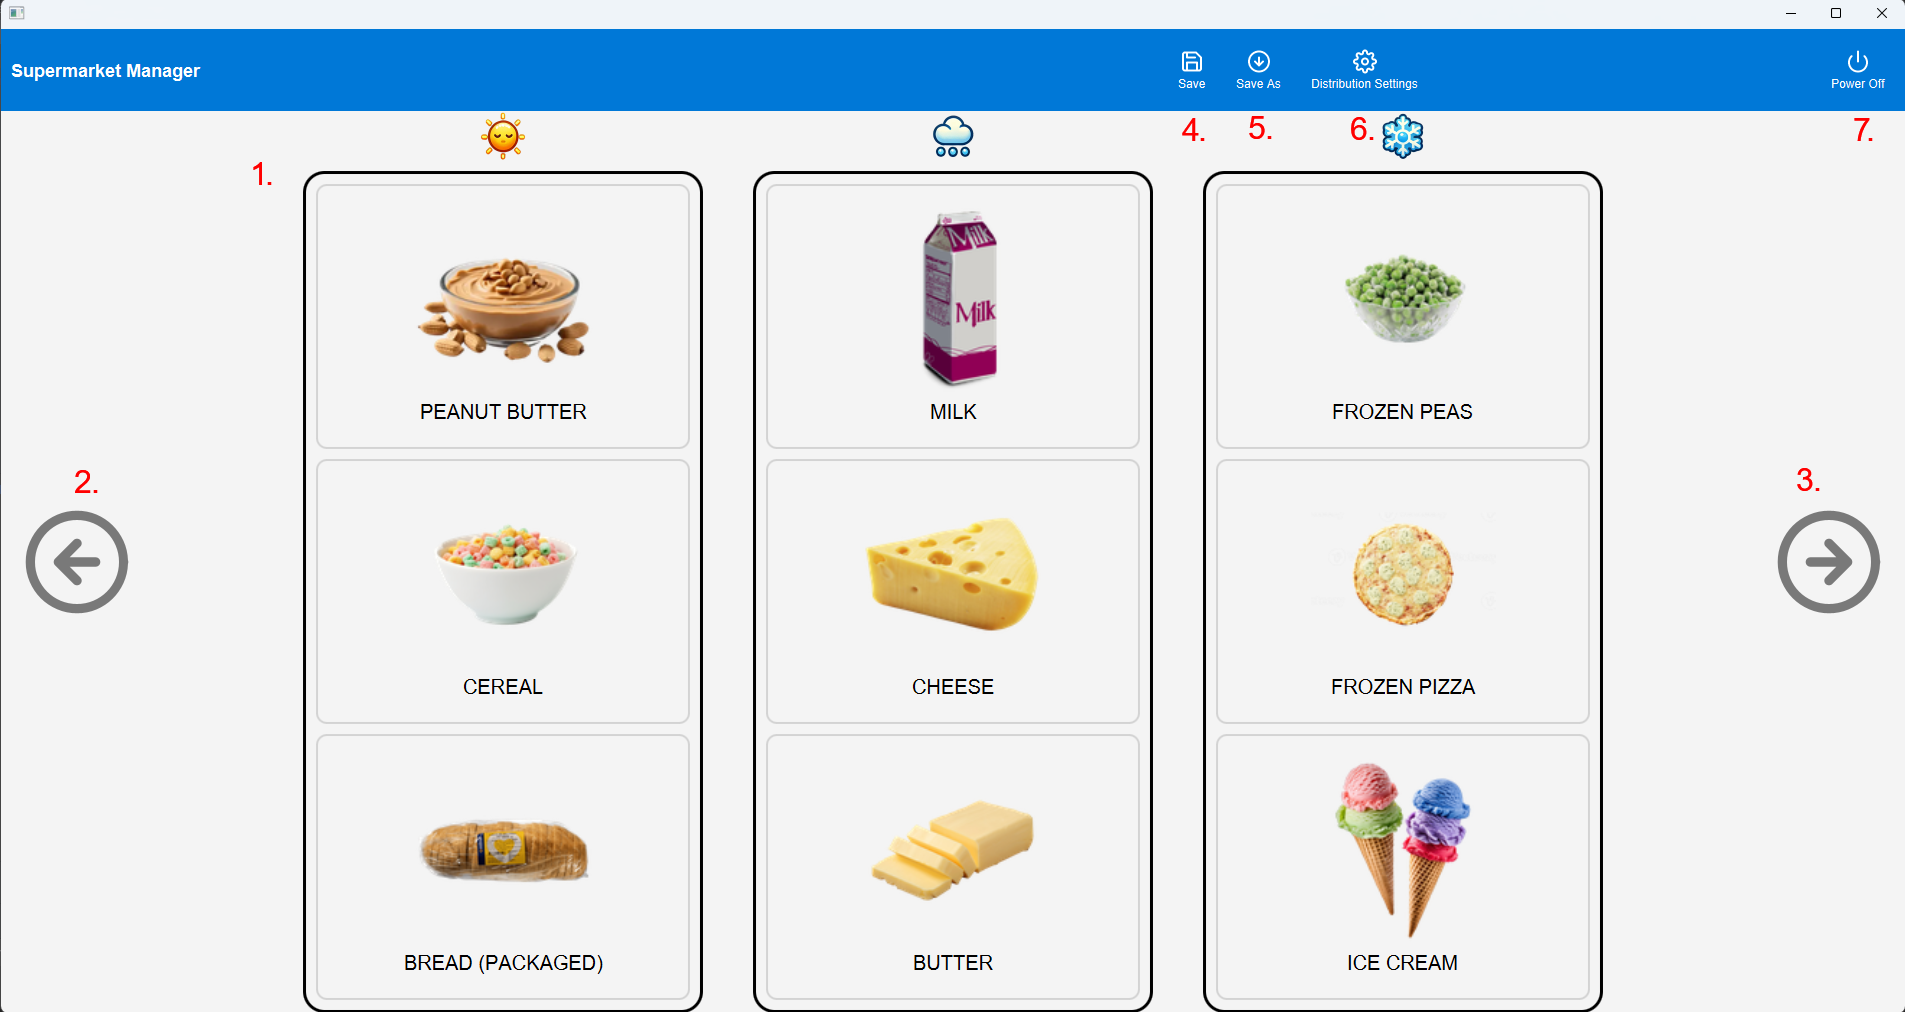
\includegraphics[width=0.75\linewidth]{assets/mainscreen.png}
		\caption{Interfície de Main Screen}
	\end{figure}
	
	\noindent Les funcionalitats de la vista són:
	
	\begin{enumerate}[itemsep=0pt, topsep=0pt]
		\item Distribució dels productes en 3 prestatgeries contingents. El número superior indica la posició de la prestatgeria.
		\item Navegar cap a la següent prestatgeria cap a l'esquerra.
		\item Navegar cap a la següent prestatgeria cap a la dreta.
		\item (\textbf{ADMIN}) Botó que permet guardar la configuració en local.
		\item (\textbf{ADMIN}) Botó per guardar la configuració en un fitxer extern.
		\item Botó per navegar al cercador de productes Catalog (\ref{sec:catalog})
		\item (\textbf{ADMIN}) Botó per configurar la distribució del supermercat, navegarem a Edit Ditribution (\ref{sec:editDistribution}).
		\item Botó per o bé tancar la app o bé per tancar sessió, que ens farà navegar a Log In (\ref{sec:logIn}).
	\end{enumerate}
	
	\newpage
	\subsection{Edit Distribution}
	\label{sec:editDistribution}
	
	La vista Edit Distribution, tal i com indica el seu nom ens permetrà modificar la distribució de productes en el supermercat. Les operacions que pot fer seran detallades a continuació. \\
	
	Tenir en compte que aquesta vista només podrà ser accedida per l'\textbf{administrador} del sistema.
	
	\begin{figure}[H] 
		\centering
		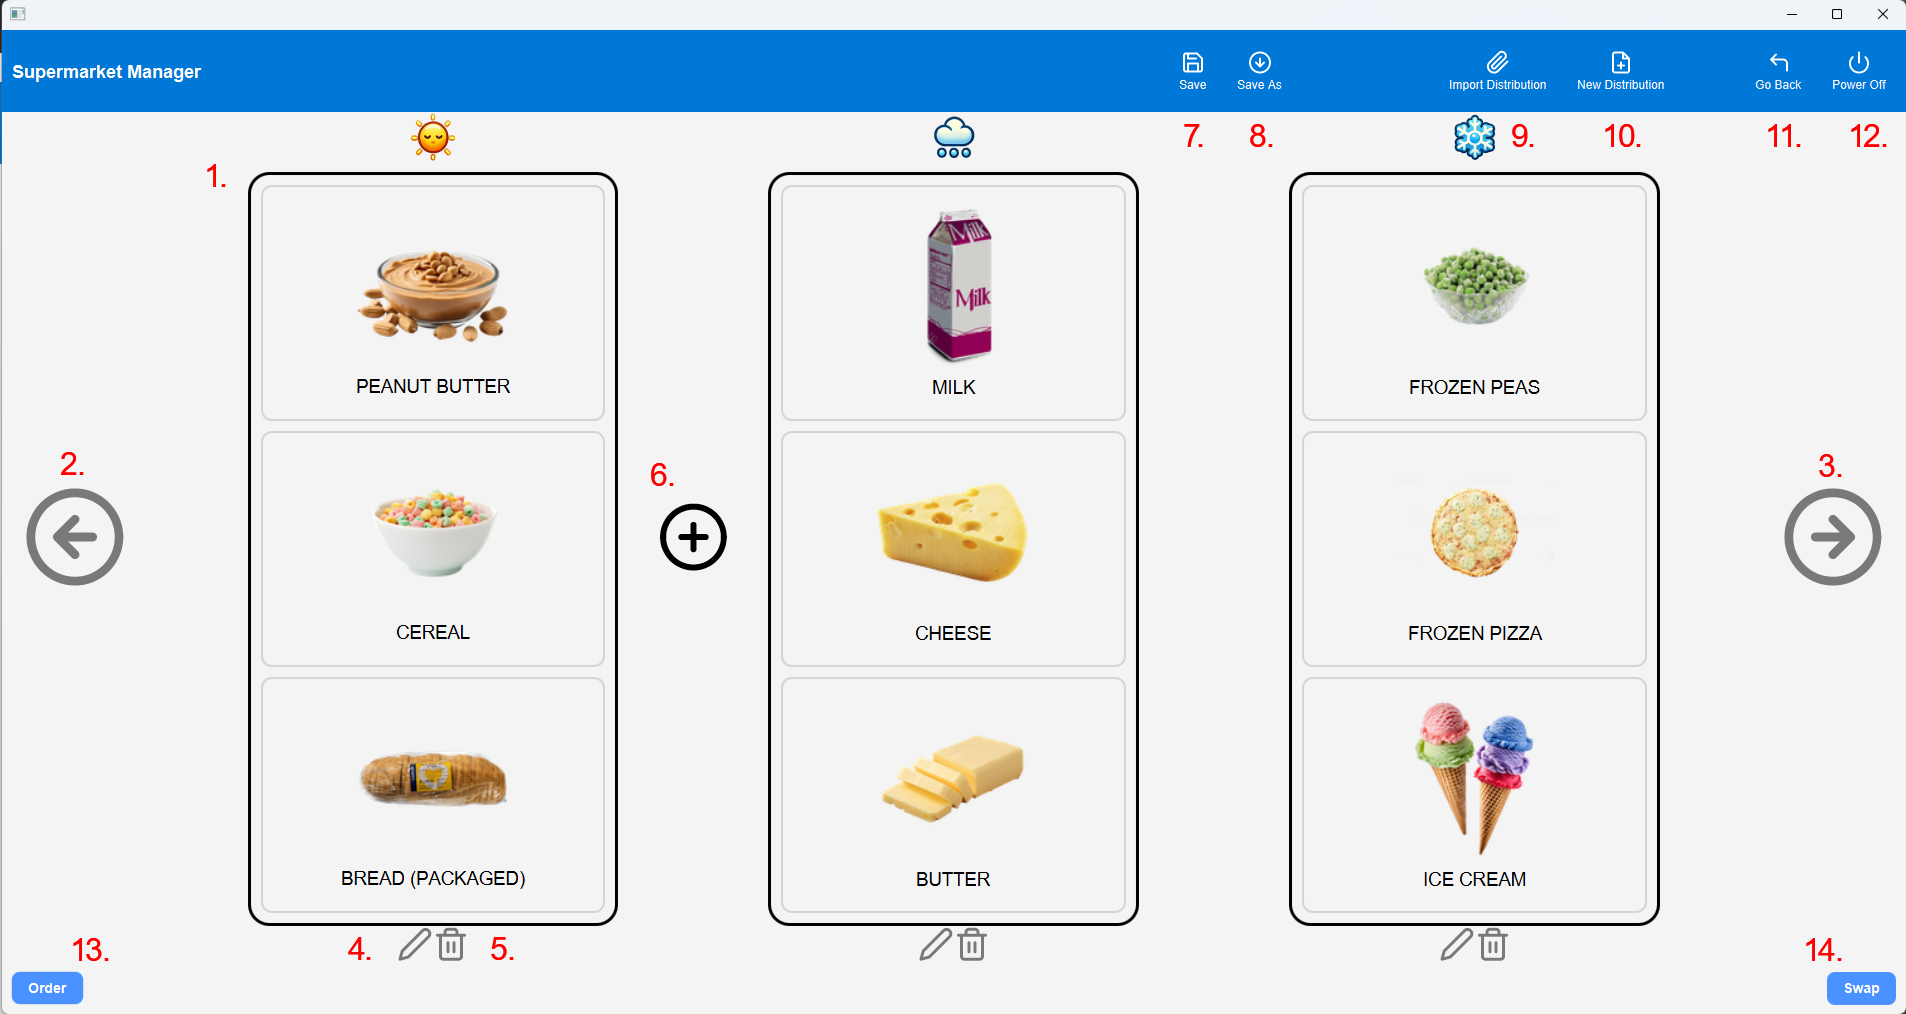
\includegraphics[width=0.75\linewidth]{assets/editdistribution.png}
		\caption{Interfície de Edit Distribution}
	\end{figure}
	
	\noindent Les funcionalitats de la vista són:
	
	\begin{enumerate}[itemsep=0pt, topsep=0pt]
		\item Distribució dels productes en 3 prestatgeries contingents.
		\item Navegar cap a la següent prestatgeria cap a l'esquerra.
		\item Navegar cap a la següent prestatgeria cap a la dreta.
		\item Editar la prestatgeria, això ens portarà a Edit Shelving Unit (\ref{sec:editShelvingUnit}).
		\item Esborrar la prestatgeria.
		\item Afegir una prestatgeria en aquella posició. Aquest botó apareix dinàmicament al apropar el cursor entre dues prestatgeries.
		\item Botó per guardar la configuració en local.
		\item Botó per guardar la configuració en un fitxer extern.
		\item Botó per navegar al cercador de productes Catalog (\ref{sec:catalog})
		\item Botó per importar una configuració externa.
		\item Botó per crear des de zero una nova configuració.
		\item Botó per anar a Main Screen (\ref{sec:mainScreen}).
		\item Botó per o bé tancar la app o bé per tancar sessió, que ens farà navegar a Log In (\ref{sec:logIn}).
		\item Botó per ordenar els productes, des de catàleg o des de supermercat, amb un dels tres mètodes disponibles (GREEDY, APROXIMATION i BACKTRACKING).
		\item Botó per intercanviar la posició de dos productes o de dos prestatgeries. En aquest punt, en tots els prestatges es dibuixarà una caixeta per seleccionar els productes que s'intercanviaran. I el mateix amb cada prestatgeria.
	\end{enumerate}
	
	\newpage
	\subsection{Edit Shelving Unit}
	\label{sec:editShelvingUnit}
	
	De la anterior visita naveguem a aquesta. La vista Edit Shelving Unit és la encarregada de facilitar la edició d'una prestatgeria. Com la anterior, aquesta vista només serà accesible per l'\textbf{administrador}.
	
	\begin{figure}[H] 
		\centering
		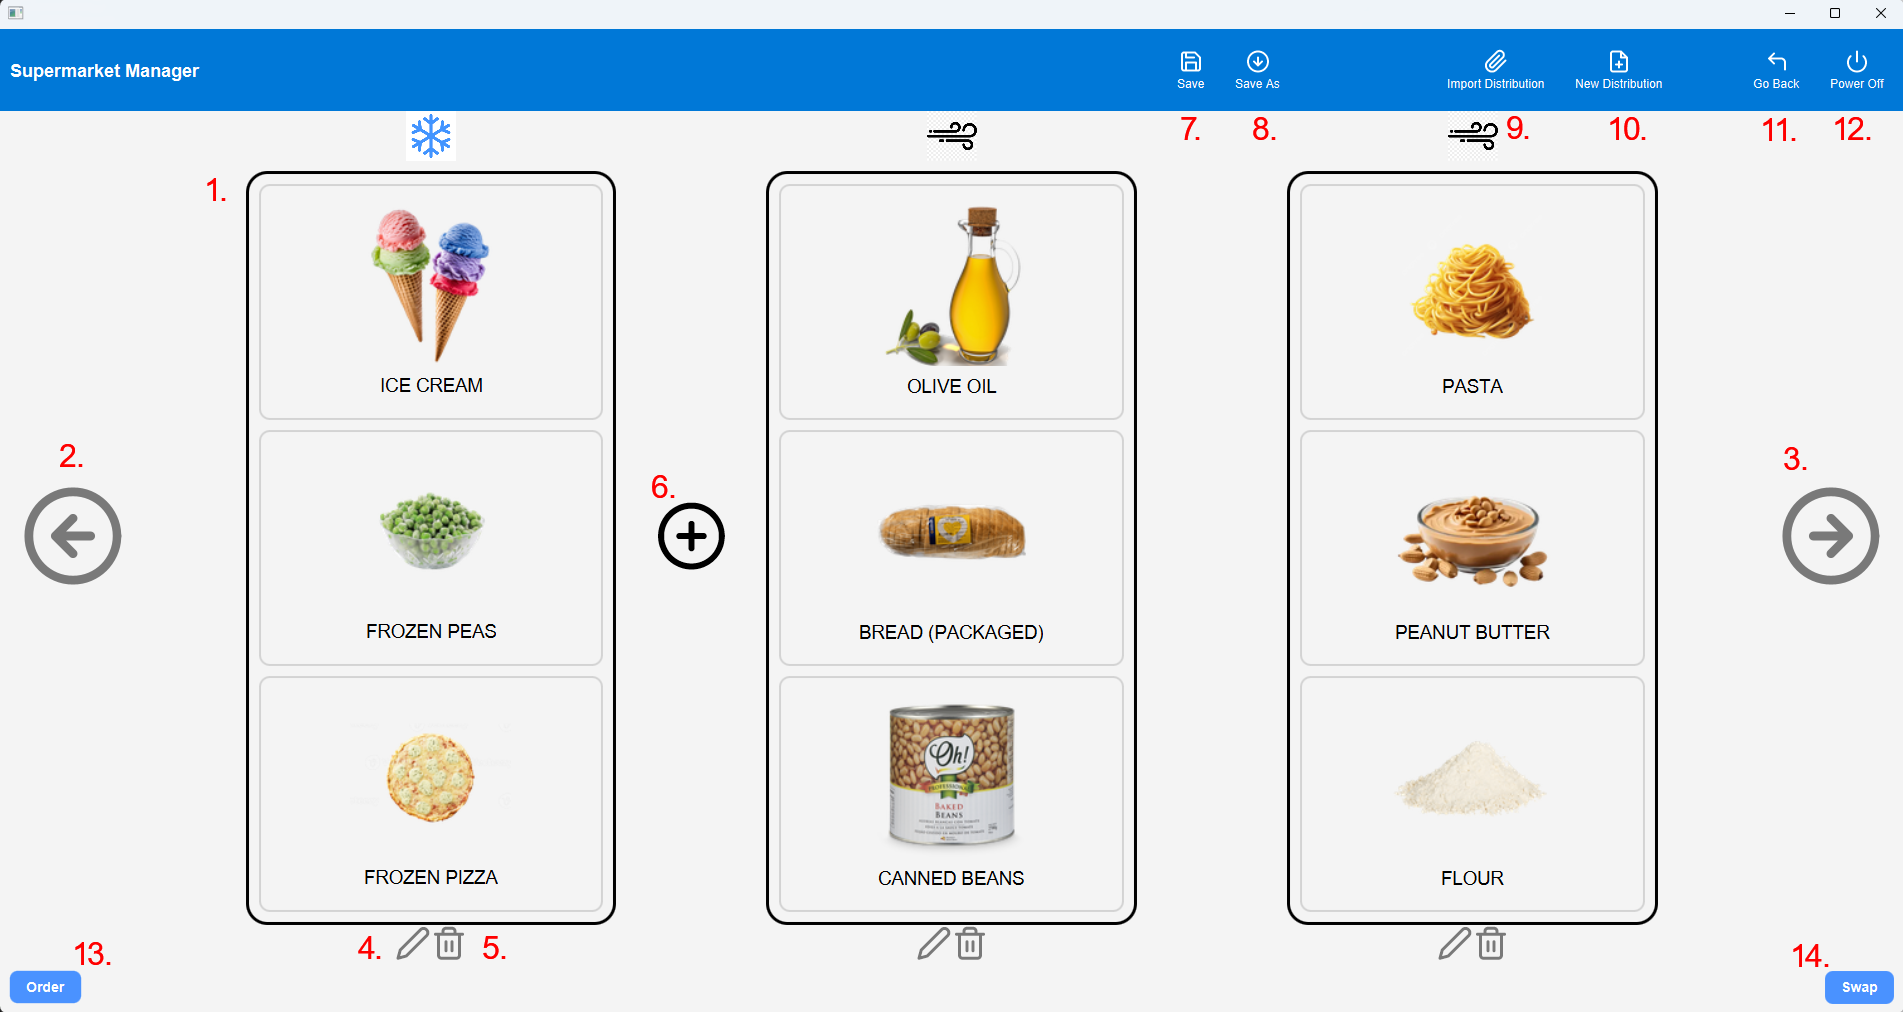
\includegraphics[width=0.75\linewidth]{assets/editshelvingunit.png}
		\caption{Interfície de Edit Shelving Unit}
	\end{figure}
	
	\noindent Les funcionalitats de la vista són:
	
	\begin{enumerate}[itemsep=0pt, topsep=0pt]
		\item Permet modificar el tipus de temperatura, per acceptar els canvis, premer el tick; per cancelar-los, la creu.
		\item Botó per buidar la prestatgeria.
		\item Botó per eliminar la prestatgeria, a continuació navegarem a Edit Distribution (\ref{sec:editDistribution}).
		\item Botó per confirmar els canvis en la prestatgeria, d'aquesta manera, amb el Go Back, podrem desfer els canvis.
		\item Distribució de productes de la prestatgeria.
		\item Esborra el producte en aquella posició.
		\item Afegeix un producte (a escollir) en aquella posició.
		\item Botó que permet guardar la configuració en local.
		\item Botó per guardar la configuració en un fitxer extern.
		\item Botó per anar a la vista anterior, Edit Distribution (\ref{sec:editDistribution}).
		\item Botó per o bé tancar la app o bé per tancar sessió, que ens farà navegar a Log In (\ref{sec:logIn}).
		
	\end{enumerate}
	
	\newpage
	\subsection{Catalog}
	\label{sec:catalog}
	
	Aquesta vista ens permet veure tots els productes, i, en cas de que siguem administradors, modificar, afegir i eliminar productes. Quan enumerem les funcionalitats, mencionarem quines son només de l'administrador amb el símbol (\textbf{ADMIN}).
	
	\begin{figure}[H] 
		\centering
		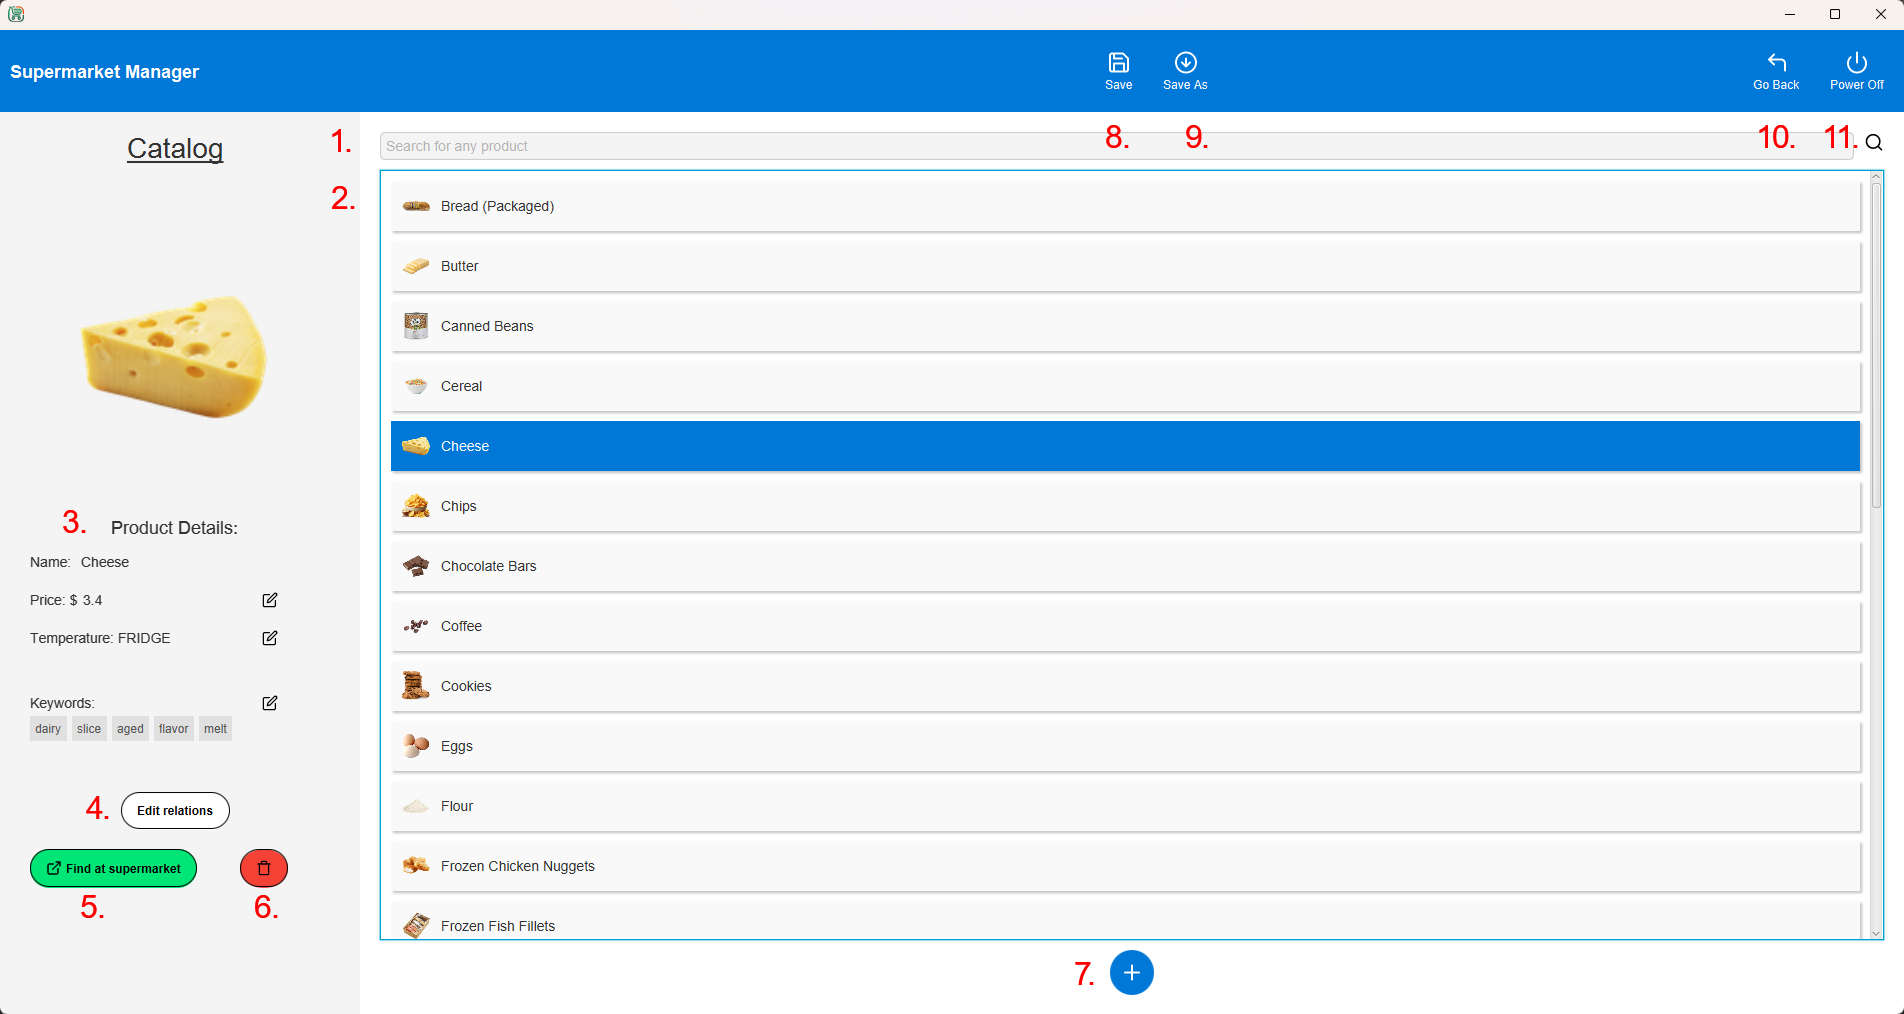
\includegraphics[width=0.75\linewidth]{assets/catalog.png}
		\caption{Interfície de Catalog}
	\end{figure}
	
	\noindent Les funcionalitats de la vista són:
	
	\begin{enumerate}[itemsep=0pt, topsep=0pt]
		\item Cercador de productes.
		\item Resultats de la cerca de productes.
		\item (\textbf{ADMIN}) Botó per modificar les relacions entre els productes. S'obrirà una pestanya amb totes les relacions del producte seleccionat amb tots els demès. Allà es podran consultar i modificar les relacions.
		\item (\textbf{ADMIN}) Edició de les relacions entre els productes.
		\item Trobar la localització del producte en el supermercat.
		\item (\textbf{ADMIN}) Eliminar el producte del catàleg.
		\item (\textbf{ADMIN}) Per crear un producte nou.
		\item (\textbf{ADMIN}) Botó que permet guardar la configuració en local.
		\item (\textbf{ADMIN}) Botó per guardar la configuració en un fitxer extern.
		\item Botó per anar a la vista anterior, Edit Distribution (\ref{sec:mainScreen}).
		\item Botó per o bé tancar la app o bé per tancar sessió, que ens farà navegar a Log In
	\end{enumerate}
	
	\newpage
	\section{Funcionalitats del programa}
	
	\subsection{Gestió de fitxers de persistència}

	Aquest sistema utilitza un únic fitxer \texttt{.json} per emmagatzemar totes les dades de la sessió. El sistema de fitxers es divideix de la següent manera:
	
	\begin{itemize}
		\item \textbf{\texttt{default.json}}: Aquest fitxer es troba als recursos del programa. És on es desaran els canvis per defecte i també el que es carregarà en fer \textit{log in}.
		\item \textbf{Altres fitxers \texttt{.json}}: L'usuari pot carregar fitxers \texttt{.json} per provar diferents configuracions amb productes diversos. No és necessari reescriure el \texttt{default.json}, ja que existeix un cas d'ús per importar un supermercat complet, que inclou tant el catàleg de productes com la seva distribució. Així mateix, l'usuari pot desar la configuració en un fitxer diferent del per defecte.
	\end{itemize}
	
	Un cop carregada la configuració del supermercat al sistema, l'usuari pot fer modificacions i guardar els canvis mitjançant les funcionalitats de \textit{Save} i \textit{Save As}. A continuació, es detalla com funciona cadascuna d'aquestes funcionalitats:
	
	\begin{itemize}
		\item \textbf{\textit{Save}}: Exporta la configuració actual del sistema, incloent-hi les modificacions realitzades per l'administrador, al fitxer \texttt{default.json}, que serà sobreescrit.
		\item \textbf{\textit{Save As}}: Obre un menú que permet a l'usuari seleccionar un directori i especificar el nom del fitxer amb l'extensió \texttt{.json} on es desarà la configuració del supermercat. Aquesta funcionalitat permet guardar la configuració amb un altre nom o en una ubicació diferent.
	\end{itemize}
	
	Si l'administrador tanca sessió sense haver desat els canvis (ni amb \textit{Save} ni amb \textit{Save As}), el sistema preguntarà si vol desar-los. Si respon afirmativament, els canvis es desaran; en cas contrari, es descartaran. \\
	
	Pel que fa al sistema d’imatges, aquest funciona de manera lleugerament diferent. La carpeta que conté les imatges associades als productes sempre serà \texttt{productImgs/<name>.png}. Quan es crea un producte nou, es demana a l'usuari que seleccioni la imatge que representarà el producte (es recomana una resolució de 128x128 píxels). Al carregar una nova configuració, les imatges dels productes han d’estar a \texttt{productImgs/<name>.png} perquè es mostrin correctament. Si no hi són, el programa mostrarà una imatge per defecte indicant que no s’ha trobat la imatge associada.

\end{document}